\documentclass[12pt,letterpaper]{article}
\usepackage{graphicx,textcomp}
\usepackage{natbib}
\usepackage{setspace}
\usepackage{fullpage}
\usepackage{color}
\usepackage[reqno]{amsmath}
\usepackage{amsthm}
\usepackage{fancyvrb}
\usepackage{amssymb,enumerate}
\usepackage[all]{xy}
\usepackage{endnotes}
\usepackage{lscape}
\newtheorem{com}{Comment}
\usepackage{float}
\usepackage{hyperref}
\newtheorem{lem} {Lemma}
\newtheorem{prop}{Proposition}
\newtheorem{thm}{Theorem}
\newtheorem{defn}{Definition}
\newtheorem{cor}{Corollary}
\newtheorem{obs}{Observation}
\usepackage[compact]{titlesec}
\usepackage{dcolumn}
\usepackage{tikz}
\usetikzlibrary{arrows}
\usepackage{multirow}
\usepackage{xcolor}
\newcolumntype{.}{D{.}{.}{-1}}
\newcolumntype{d}[1]{D{.}{.}{#1}}
\definecolor{light-gray}{gray}{0.65}
\usepackage{url}
\usepackage{listings}
\usepackage{color}

\definecolor{codegreen}{rgb}{0,0.6,0}
\definecolor{codegray}{rgb}{0.5,0.5,0.5}
\definecolor{codepurple}{rgb}{0.58,0,0.82}
\definecolor{backcolour}{rgb}{0.95,0.95,0.92}

\lstdefinestyle{mystyle}{
	backgroundcolor=\color{backcolour},   
	commentstyle=\color{codegreen},
	keywordstyle=\color{magenta},
	numberstyle=\tiny\color{codegray},
	stringstyle=\color{codepurple},
	basicstyle=\footnotesize,
	breakatwhitespace=false,         
	breaklines=true,                 
	captionpos=b,                    
	keepspaces=true,                 
	numbers=left,                    
	numbersep=5pt,                  
	showspaces=false,                
	showstringspaces=false,
	showtabs=false,                  
	tabsize=2
}
\lstset{style=mystyle}
\newcommand{\Sref}[1]{Section~\ref{#1}}
\newtheorem{hyp}{Hypothesis}

\title{Problem Set 3}
\date{Due: November 11, 2024}
\author{Applied Stats/Quant Methods 1}


\begin{document}
	\maketitle
	\section*{Instructions}
	\begin{itemize}
		\item Please show your work! You may lose points by simply writing in the answer. If the problem requires you to execute commands in \texttt{R}, please include the code you used to get your answers. Please also include the \texttt{.R} file that contains your code. If you are not sure if work needs to be shown for a particular problem, please ask.
	\item Your homework should be submitted electronically on GitHub.
	\item This problem set is due before 23:59 on Sunday November 11, 2024. No late assignments will be accepted.

	\end{itemize}

		\vspace{.25cm}
	
\noindent In this problem set, you will run several regressions and create an add variable plot (see the lecture slides) in \texttt{R} using the \texttt{incumbents\_subset.csv} dataset. Include all of your code.

	\vspace{.5cm}
	\newpage
\section*{Question 1}
\vspace{.25cm}
\noindent We are interested in knowing how the difference in campaign spending between incumbent and challenger affects the incumbent's vote share. 
	\lstinputlisting[language=R, firstline=42, lastline=43]{PS03_AnswersDH.R}
	
	\begin{enumerate}
		\item Run a regression where the outcome variable is \texttt{voteshare} and the explanatory variable is
		\texttt{difflog}.
		\lstinputlisting[language=R, firstline=50, lastline=51]{PS03_AnswersDH.R}
		\begin{table}[!htbp] \centering 
			\caption{} 
			\label{} 
			\begin{tabular}{@{\extracolsep{5pt}}lc} 
				\\[-1.8ex]\hline 
				\hline \\[-1.8ex] 
				& \multicolumn{1}{c}{\textit{Dependent variable:}} \\ 
				\cline{2-2} 
				\\[-1.8ex] & voteshare \\ 
				\hline \\[-1.8ex] 
				difflog & 0.042$^{***}$ \\ 
				& (0.001) \\ 
				& \\ 
				Constant & 0.579$^{***}$ \\ 
				& (0.002) \\ 
				& \\ 
				\hline \\[-1.8ex] 
				Observations & 3,193 \\ 
				R$^{2}$ & 0.367 \\ 
				Adjusted R$^{2}$ & 0.367 \\ 
				Residual Std. Error & 0.079 (df = 3191) \\ 
				F Statistic & 1,852.791$^{***}$ (df = 1; 3191) \\ 
				\hline 
				\hline \\[-1.8ex] 
				\textit{Note:}  & \multicolumn{1}{r}{$^{*}$p$<$0.1; $^{**}$p$<$0.05; $^{***}$p$<$0.01} \\ 
			\end{tabular} 
		\end{table}

		 \vspace*{0.5cm}
		\noindent
		On average, a one unit increase in the logged difference in campaign spending is associated with a 4.2\% increase in the incumbent vote share. The positive correlation between the two variables is statistically reliable. 
		
		\newpage
		\item Make a scatterplot of the two variables and add the regression line. 	
	\lstinputlisting[language=R, firstline=55, lastline=63]{PS03_AnswersDH.R}
		\begin{figure}[h!]
		\centering
		\caption{\footnotesize}
		\label{fig:plot_1}
		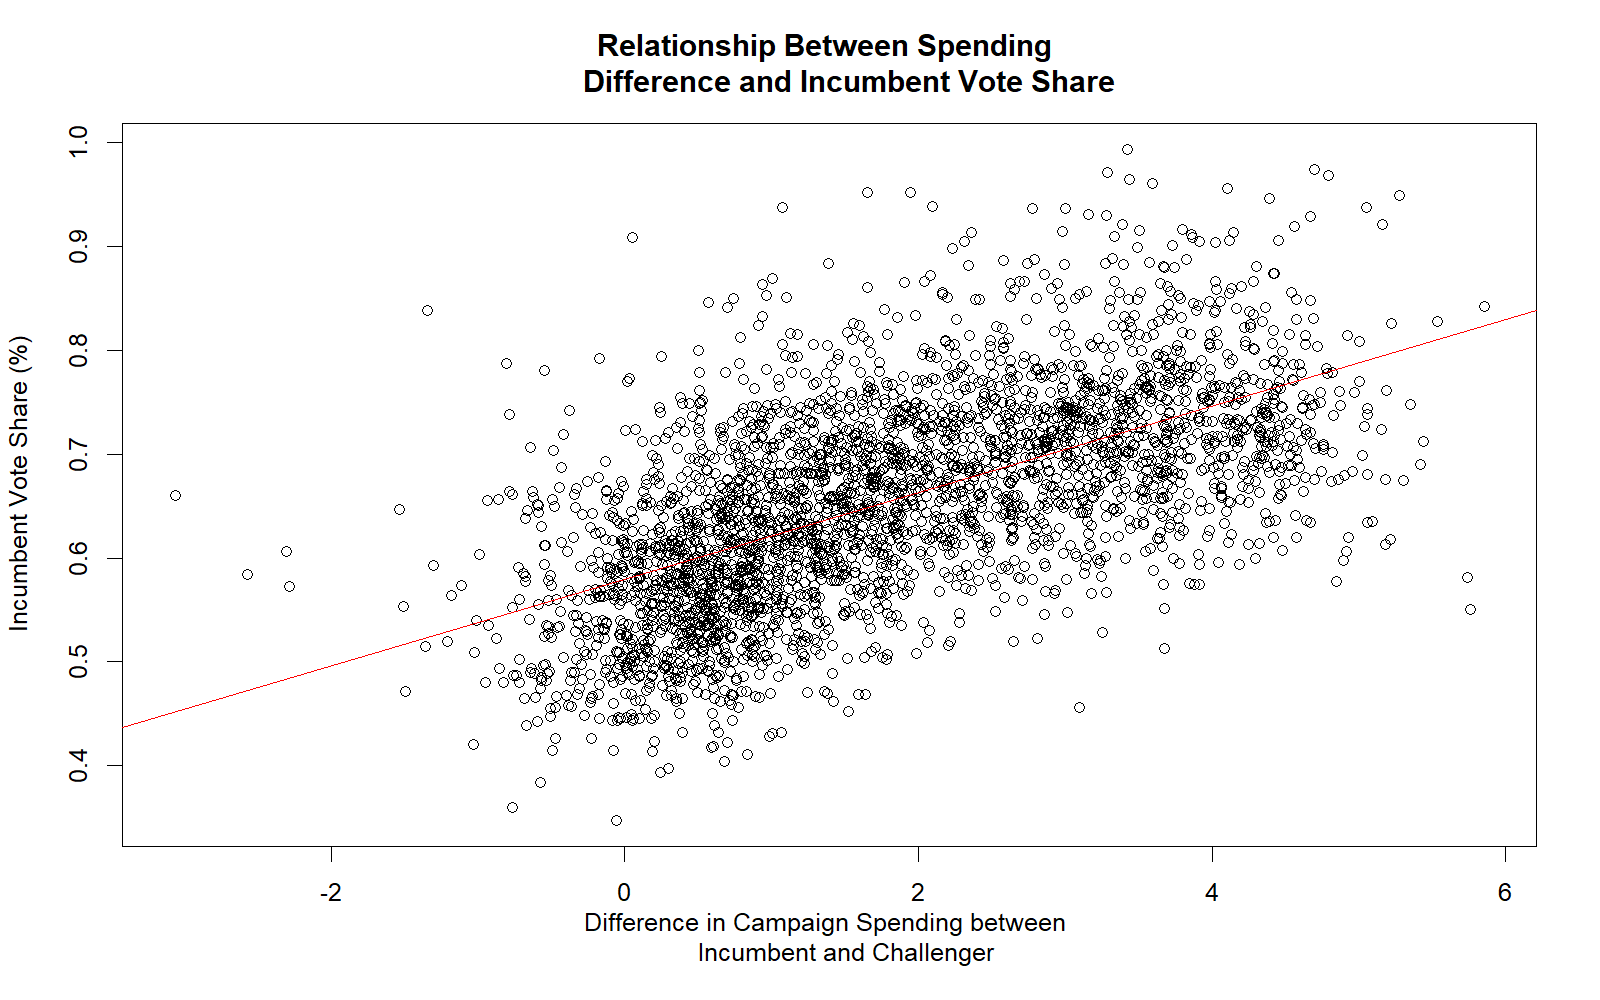
\includegraphics[width=0.85\textwidth]{Plot1}  
	\end{figure}
	\newpage
		\item Save the residuals of the model in a separate object.	\lstinputlisting[language=R, firstline=66, lastline=68]{PS03_AnswersDH.R}\vspace{4cm}
		\item Write the prediction equation.
		
		\noindent 
		
		voteshare = 0.579 + 0.042difflog 
	\end{enumerate}
	
\newpage

\section*{Question 2}
\noindent We are interested in knowing how the difference between incumbent and challenger's spending and the vote share of the presidential candidate of the incumbent's party are related.	\vspace{.25cm}
	\begin{enumerate}
		\item Run a regression where the outcome variable is \texttt{presvote} and the explanatory variable is \texttt{difflog}.	
		\lstinputlisting[language=R, firstline=79, lastline=80]{PS03_AnswersDH.R}
		\begin{table}[!htbp] \centering 
			\caption{} 
			\label{} 
			\begin{tabular}{@{\extracolsep{5pt}}lc} 
				\\[-1.8ex]\hline 
				\hline \\[-1.8ex] 
				& \multicolumn{1}{c}{\textit{Dependent variable:}} \\ 
				\cline{2-2} 
				\\[-1.8ex] & presvote \\ 
				\hline \\[-1.8ex] 
				difflog & 0.024$^{***}$ \\ 
				& (0.001) \\ 
				& \\ 
				Constant & 0.508$^{***}$ \\ 
				& (0.003) \\ 
				& \\ 
				\hline \\[-1.8ex] 
				Observations & 3,193 \\ 
				R$^{2}$ & 0.088 \\ 
				Adjusted R$^{2}$ & 0.088 \\ 
				Residual Std. Error & 0.110 (df = 3191) \\ 
				F Statistic & 307.715$^{***}$ (df = 1; 3191) \\ 
				\hline 
				\hline \\[-1.8ex] 
				\textit{Note:}  & \multicolumn{1}{r}{$^{*}$p$<$0.1; $^{**}$p$<$0.05; $^{***}$p$<$0.01} \\ 
			\end{tabular} 
		\end{table} 
		\noindent
		On average, a 1 unit increase in the logged difference in campaign spending is associated with a 2.4\% increase in the incumbent party candidates vote share. The positive correlation between the variables is statistically reliable.
		\newpage
		\item Make a scatterplot of the two variables and add the regression line. 
			\lstinputlisting[language=R, firstline=83, lastline=91]{PS03_AnswersDH.R}
				\begin{figure}[h!]
			\centering
			\caption{\footnotesize}
			\label{fig:plot_2}
			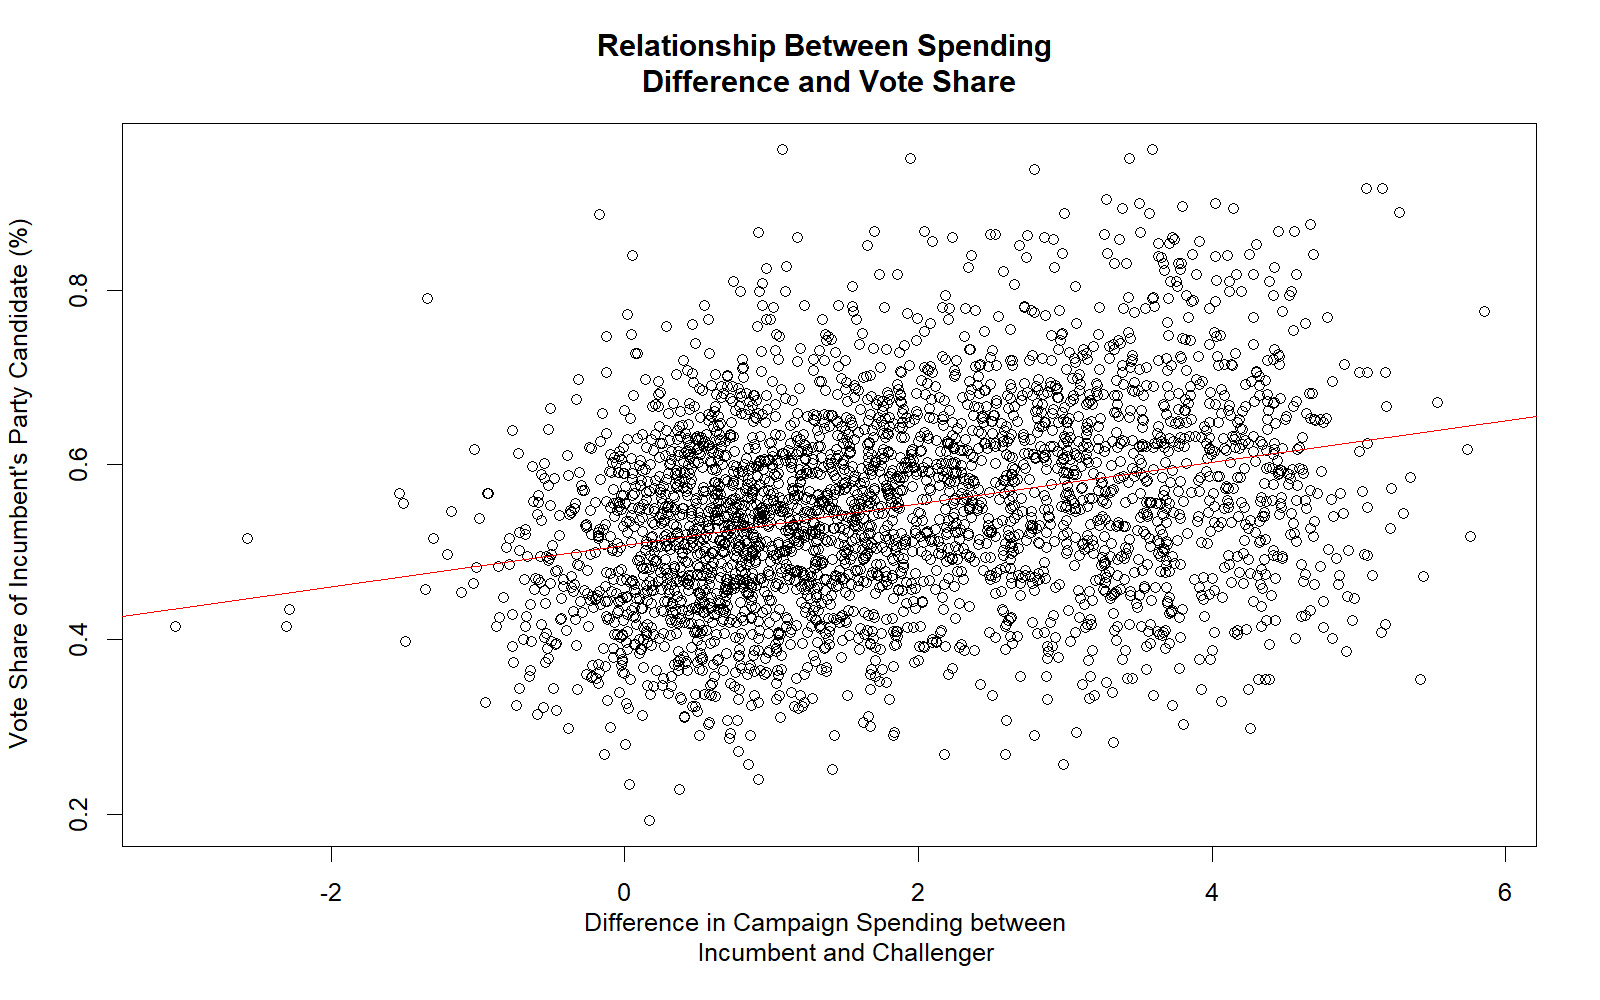
\includegraphics[width=0.85\textwidth]{Plot2}  
		\end{figure}	\vspace{2cm}
		\item Save the residuals of the model in a separate object. \lstinputlisting[language=R, firstline=94, lastline=95]{PS03_AnswersDH.R}	\vspace{0.5cm}
		\item Write the prediction equation.
		\noindent 
		
		presvote = 0.508 + 0.024difflog 
	\end{enumerate}
	
	\newpage	
\section*{Question 3}

\noindent We are interested in knowing how the vote share of the presidential candidate of the incumbent's party is associated with the incumbent's electoral success.
	\vspace{.25cm}
	\begin{enumerate}
		\item Run a regression where the outcome variable is \texttt{voteshare} and the explanatory variable is \texttt{presvote}
		\lstinputlisting[language=R, firstline=105, lastline=106]{PS03_AnswersDH.R}.
		\begin{table}[!htbp] \centering 
			\caption{} 
			\label{} 
			\begin{tabular}{@{\extracolsep{5pt}}lc} 
				\\[-1.8ex]\hline 
				\hline \\[-1.8ex] 
				& \multicolumn{1}{c}{\textit{Dependent variable:}} \\ 
				\cline{2-2} 
				\\[-1.8ex] & voteshare \\ 
				\hline \\[-1.8ex] 
				presvote & 0.388$^{***}$ \\ 
				& (0.013) \\ 
				& \\ 
				Constant & 0.441$^{***}$ \\ 
				& (0.008) \\ 
				& \\ 
				\hline \\[-1.8ex] 
				Observations & 3,193 \\ 
				R$^{2}$ & 0.206 \\ 
				Adjusted R$^{2}$ & 0.206 \\ 
				Residual Std. Error & 0.088 (df = 3191) \\ 
				F Statistic & 826.950$^{***}$ (df = 1; 3191) \\ 
				\hline 
				\hline \\[-1.8ex] 
				\textit{Note:}  & \multicolumn{1}{r}{$^{*}$p$<$0.1; $^{**}$p$<$0.05; $^{***}$p$<$0.01} \\ 
			\end{tabular} 
		\end{table} \vspace{3cm}
		
		\noindent
		On average, a one unit increase in the incumbent party candidates vote share is associated with a 38.8\% increase in the incumbent vote share. The positive correlation between the two variables is statistically reliable.
		
		\newpage
		\item Make a scatterplot of the two variables and add the regression line.
		 	\lstinputlisting[language=R, firstline=109, lastline=116]{PS03_AnswersDH.R}
						\begin{figure}[h!]
			\centering
			\caption{\footnotesize}
			\label{fig:plot_3}
			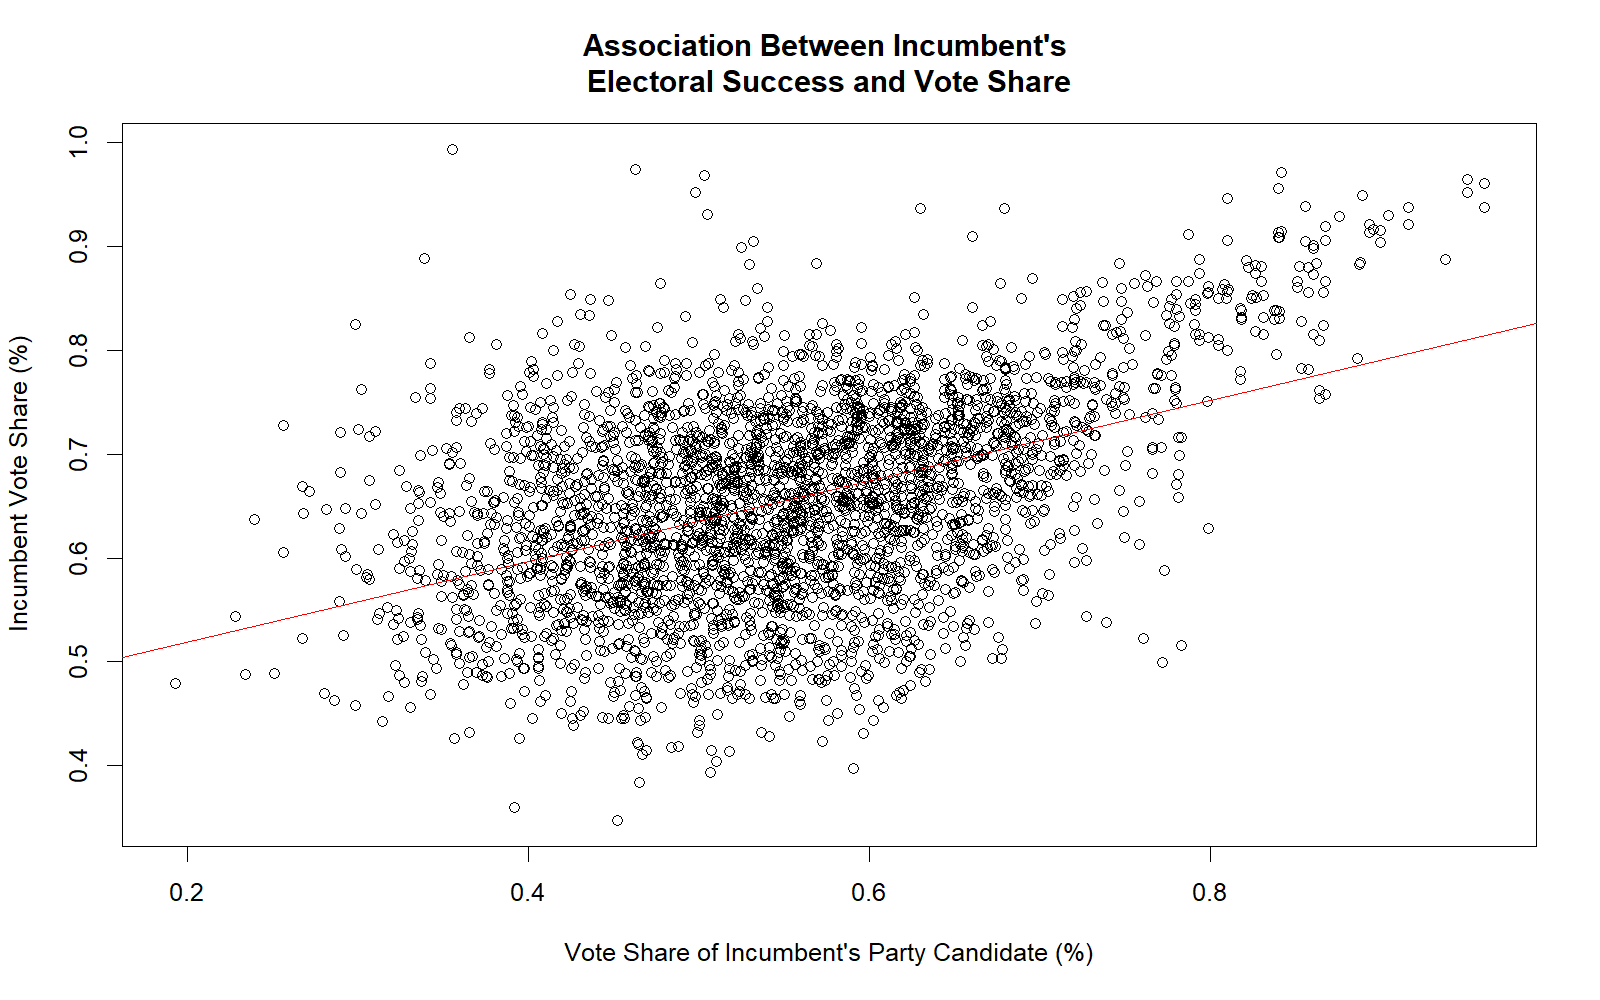
\includegraphics[width=0.85\textwidth]{Plot3}  
		\end{figure} 
			\vspace{2cm}
		\item Write the prediction equation.
		\noindent 
		
		voteshare = 0.441 + 0.388presvote
	\end{enumerate}
	

\newpage	
\section*{Question 4}
\noindent The residuals from part (a) tell us how much of the variation in \texttt{voteshare} is $not$ explained by the difference in spending between incumbent and challenger. The residuals in part (b) tell us how much of the variation in \texttt{presvote} is $not$ explained by the difference in spending between incumbent and challenger in the district.
	\begin{enumerate}
		\item Run a regression where the outcome variable is the residuals from Question 1 and the explanatory variable is the residuals from Question 2.
		\lstinputlisting[language=R, firstline=126, lastline=127]{PS03_AnswersDH.R}	
		\begin{table}[!htbp] \centering 
			\caption{} 
			\label{} 
			\begin{tabular}{@{\extracolsep{5pt}}lc} 
				\\[-1.8ex]\hline 
				\hline \\[-1.8ex] 
				& \multicolumn{1}{c}{\textit{Dependent variable:}} \\ 
				\cline{2-2} 
				\\[-1.8ex] & residuals\_model1 \\ 
				\hline \\[-1.8ex] 
				residuals\_model2 & 0.257$^{***}$ \\ 
				& (0.012) \\ 
				& \\ 
				Constant & $-$0.000 \\ 
				& (0.001) \\ 
				& \\ 
				\hline \\[-1.8ex] 
				Observations & 3,193 \\ 
				R$^{2}$ & 0.130 \\ 
				Adjusted R$^{2}$ & 0.130 \\ 
				Residual Std. Error & 0.073 (df = 3191) \\ 
				F Statistic & 476.975$^{***}$ (df = 1; 3191) \\ 
				\hline 
				\hline \\[-1.8ex] 
				\textit{Note:}  & \multicolumn{1}{r}{$^{*}$p$<$0.1; $^{**}$p$<$0.05; $^{***}$p$<$0.01} \\ 
			\end{tabular} 
			
			\vspace{1.5cm}
			
			\noindent
			On average, a one unit increase in the residuals of model 2 is associated with a 0.257 unit increase in the residuals of model 1. The positive correlation between the variables is statistically reliable.
	
		\end{table} \vspace{6cm}
		\newpage
		\item Make a scatterplot of the two residuals and add the regression line.
 	\lstinputlisting[language=R, firstline=130, lastline=136]{PS03_AnswersDH.R}
		\begin{figure}[h!]
			\centering
			\caption{\footnotesize}
			\label{fig:plot_4}
			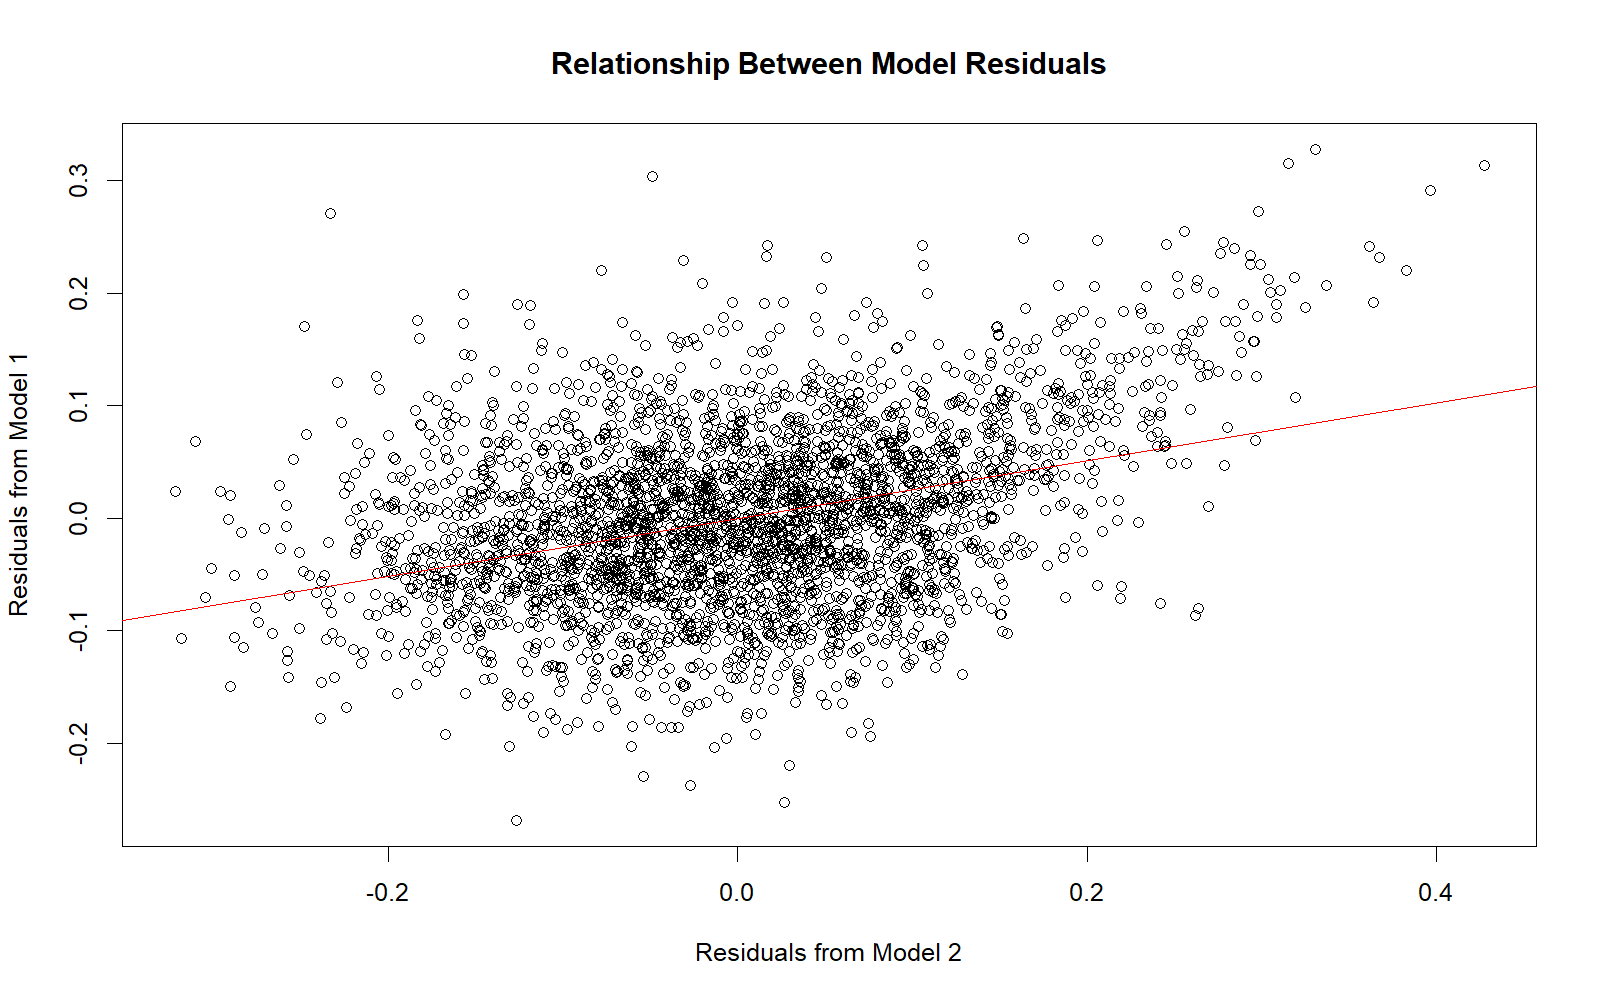
\includegraphics[width=0.85\textwidth]{Plot4}  
		\end{figure} 	\vspace{2cm}
		\item Write the prediction equation.
		\noindent
		
		residuals model 1 = -0.000 + 0.257residualsmodel2
	\end{enumerate}
	
	\newpage	

\section*{Question 5}
\noindent What if the incumbent's vote share is affected by both the president's popularity and the difference in spending between incumbent and challenger? 
	\begin{enumerate}
		\item Run a regression where the outcome variable is the incumbent's \texttt{voteshare} and the explanatory variables are \texttt{difflog} and \texttt{presvote}.	
		\lstinputlisting[language=R, firstline=147, lastline=148]{PS03_AnswersDH.R}	
		\begin{table}[!htbp] \centering 
			\caption{} 
			\label{} 
			\begin{tabular}{@{\extracolsep{5pt}}lc} 
				\\[-1.8ex]\hline 
				\hline \\[-1.8ex] 
				& \multicolumn{1}{c}{\textit{Dependent variable:}} \\ 
				\cline{2-2} 
				\\[-1.8ex] & voteshare \\ 
				\hline \\[-1.8ex] 
				difflog & 0.036$^{***}$ \\ 
				& (0.001) \\ 
				& \\ 
				presvote & 0.257$^{***}$ \\ 
				& (0.012) \\ 
				& \\ 
				Constant & 0.449$^{***}$ \\ 
				& (0.006) \\ 
				& \\ 
				\hline \\[-1.8ex] 
				Observations & 3,193 \\ 
				R$^{2}$ & 0.450 \\ 
				Adjusted R$^{2}$ & 0.449 \\ 
				Residual Std. Error & 0.073 (df = 3190) \\ 
				F Statistic & 1,302.947$^{***}$ (df = 2; 3190) \\ 
				\hline 
				\hline \\[-1.8ex] 
				\textit{Note:}  & \multicolumn{1}{r}{$^{*}$p$<$0.1; $^{**}$p$<$0.05; $^{***}$p$<$0.01} \\ 
			\end{tabular} 
		\end{table} \vspace{2cm}
		\noindent
		Holding all other variables constant, a one unit increase in the logged spending difference is associated with a 3.6\% increase in the incumbent vote share on average.
		
		Holding all other variables constant, a one unit increase in the incumbent party candidates vote share is associated with a 25.7\% increase in the incumbent's vote share on average. 
		
		Both explanatory variables have statistically reliable positive correlations with the outcome variable
		
		\item Write the prediction equation.
		
		voteshare = 0.449 + 0.036difflog + 0.257presvote	
		\vspace*{2cm}
		\item What is it in this output that is identical to the output in Question 4? Why do you think this is the case?
		\vspace*{0.5cm}
		\noindent
		
		The coefficient on the X variable "presvote" is the same as the coefficient of the residuals of model 2 when regressed on the residuals of model 1. The effect of presvote on voteshare is therefore contained within the residuals of model 2. By adding presvote to the regression model, we are therefore  removing some portion of omitted variable bias that is present within model 2 - wherein presvote was not included as a regressor.
		

	\end{enumerate}




\end{document}
